\chapter{Implementação e testes}
\label{cap:implementacaoresultados}

Neste capítulo será descrito o ambiente de alta disponibilidade que foi desenvolvido neste trabalho. Posteriormente, será apresentada a 
metodologia de testes utilizada, bem como os resultados obtidos.

\section{Descrição do ambiente de alta disponibilidade}
\label{section:implementacao}

%Para implementação desta solução foram necessários dois servidores físicos, sendo que a configuração ideal de cada servidor é de 
%real = 11 \textit{cores} de processamento, 12 GB de memória \ac{RAM} e 156 GB de disco rígido
%12 \textit{cores} de processamento, 14 GB de memória \ac{RAM} e 180 GB de disco rígido. Essa configuração foi calculada a partir da soma dos 
%recursos das máquinas virtuais que atualmente abrangem os serviços que foram considerados críticos, observa-se que tais recursos de 
%\textit{hardware} já encontravam-se disponíveis, sendo necessário somente efetuar uma reorganização das máquinas virtuais. Com essa solução, 
%caso ocorra alguma falha em um servidor, as máquinas virtuais serão transferidas para o outro servidor.

O ambiente foi projetado na forma de um \textit{cluster}, o qual é composto por dois servidores com requisitos de configuração sugeridos
de 12 \textit{cores} de processamento, 14 GB de memória \ac{RAM} e 180 GB de disco rígido.
%real = 11 \textit{cores} de processamento, 12 GB de memória \ac{RAM} e 156 GB de disco rígido
Essa configuração foi calculada a partir da soma dos recursos consumidos pelas máquinas virtuais, as quais executavam os serviços que foram 
considerados críticos. Observa-se que tais recursos de \textit{hardware} já encontravam-se disponíveis, sendo necessário somente efetuar uma 
reorganização das máquinas virtuais. Destaca-se que a configuração também inclui 2 GB de memória \ac{RAM} e 24 GB de disco para cada sistema 
operacional hóspede.

Para o desenvolvimento deste ambiente optou-se por utilizar o mesmo sistema operacional e o mesmo hipervisor que já eram utilizados na empresa, 
que são, o sistema \textit{Ubuntu 14.04 \ac{LTS}} e o \ac{KVM} \cite{kvm}, respectivamente. O processo de instalação e de configuração do sistema 
operacional e do hipervisor encontram-se no Apêndice \ref{ap:confos} e \ref{ap:confvirt}.

\subsection{Estrutura física}

A estrutura física adotada é apresentada na Figura \ref{fig:projeto_fisico} (a). Como pode ser observado, os dois servidores encontram-se 
conectados a um \textit{switch} através de dois cabos \aca{UTP}, de forma a implementar uma redundância de cabeamento. Além disso, manteve-se o 
\textit{link aggregation} e utilizou-se uma \textit{bridge}\footnote[1]{\textit{Bridges}, também conhecidas como pontes, são meios que fazem a 
conexão entre \textit{LANs}, e operam na camada de enlace de dados.} para incluir as máquinas virtuais à rede dos servidores da empresa. 
Os detalhes da configuração de rede estão localizados no Apêndice \ref{ap:confrede}.

Na Figura \ref{fig:projeto_fisico} (b) tem-se a imagem dos servidores utilizados, sendo que o primeiro é o Nó 1 (\textit{Brina}), que é um servidor
\textit{Dell PowerEdge 2950}, que possui 2 processadores \textit{Intel Xeon E5410 de 2.33 GHz}, 24 GB de memória \ac{RAM} e 1,5 TB de disco. 
Já o segundo servidor é o Nó 2 (\textit{Piova}), que é um servidor \textit{Dell PowerEdge R410}, que possui 2 processadores 
\textit{Intel Xeon E5530 de 2.40 GHz}, 32 GB de memória \ac{RAM} e 1,4 TB de disco.

\begin{figure}[h!]
 \centering
 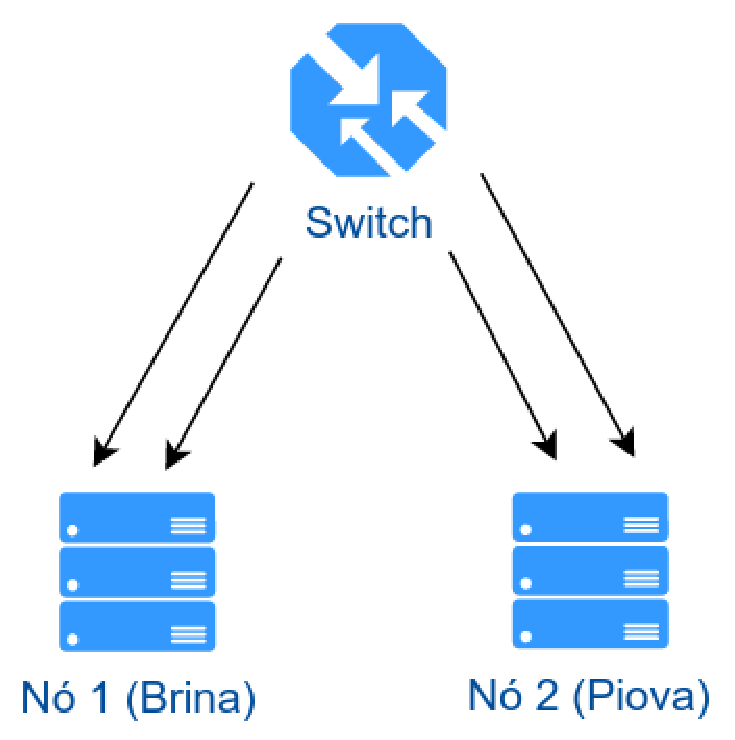
\includegraphics[width=450px]{img/projeto_fisico.eps}
 \caption{Estrutura física.}
 \label{fig:projeto_fisico}
\end{figure}

\subsection{Estrutura lógica}

A estrutura lógica do ambiente de alta disponibilidade é apresentada na Figura \ref{fig:projeto_vms}. Observa-se nessa figura que os dados são
replicados entre os nós do \textit{cluster}. Além disso, pode-se observar a distribuição dos serviços críticos entre os servidores, sendo que 
no Nó 1 foram instalados os serviços de sistemas de gestão e autenticação \ac{PPPoE}. Já no Nó 2 foram instalados os serviços de \ac{DNS} 
recursivo, telefonia e autenticação \ac{PPPoE}. No caso de falha em um nó, os serviços serão inicializados no outro nó disponível. 

\begin{figure}[h!]
 \centering
 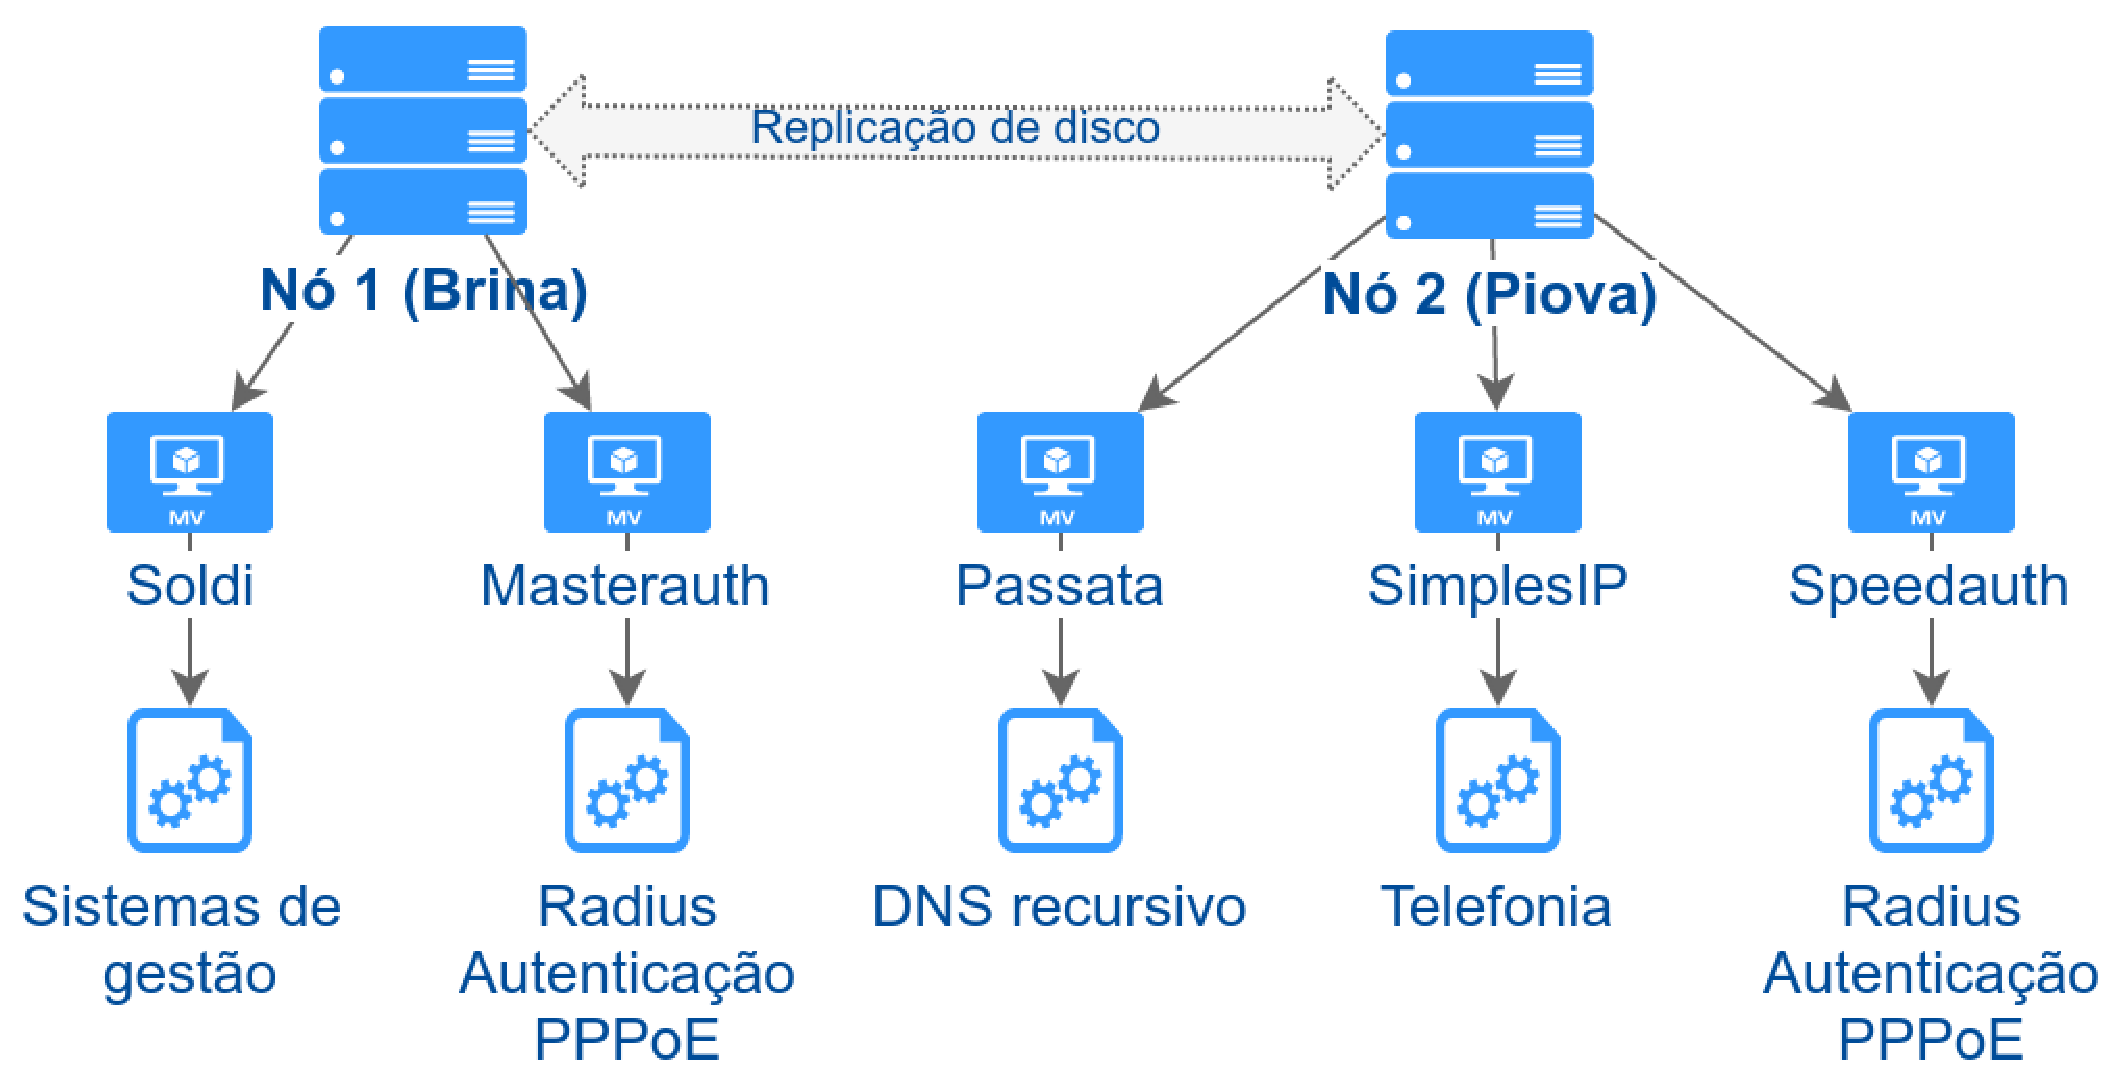
\includegraphics[width=330px]{img/projeto_vms.eps}
 \caption{Estrutura do \textit{cluster} e das máquinas virtuais.}
 \label{fig:projeto_vms}
\end{figure}

A Figura \ref{fig:projeto_estrutura} apresenta os principais componentes e \textit{softwares} que compõem o \textit{cluster} de alta 
disponibilidade. Observa-se que para o gerenciamento e monitoramento do \textit{cluster} e das \acp{VM} utilizou-se o \textit{software} 
\textit{Pacemaker}. Mais especificamente, esse é o \textit{software} responsável pelo monitoramento e pela migração das \acp{VM} entre os nós. 
Além disso, esse é responsável pelo monitoramento e gerência do \ac{DRBD}, do sistema de arquivos e das \acp{VM}. De fato, esse \textit{software} 
inicializa os serviços de acordo com a configuração definida. Por exemplo, ao inicializar o sistema operacional de um nó do \textit{cluster}, 
o \textit{Pacemaker} irá inicializar o serviço de sincronismo do \ac{DRBD}, montar o sistema de arquivos no diretório onde está localizado os 
discos das \acp{VM}, e inicializar as máquinas virtuais. O detalhamento da configuração do \textit{Pacemaker} estão disponíveis no 
Apêndice \ref{ap:confpacemaker}.

\begin{figure}[h!]
 \centering
 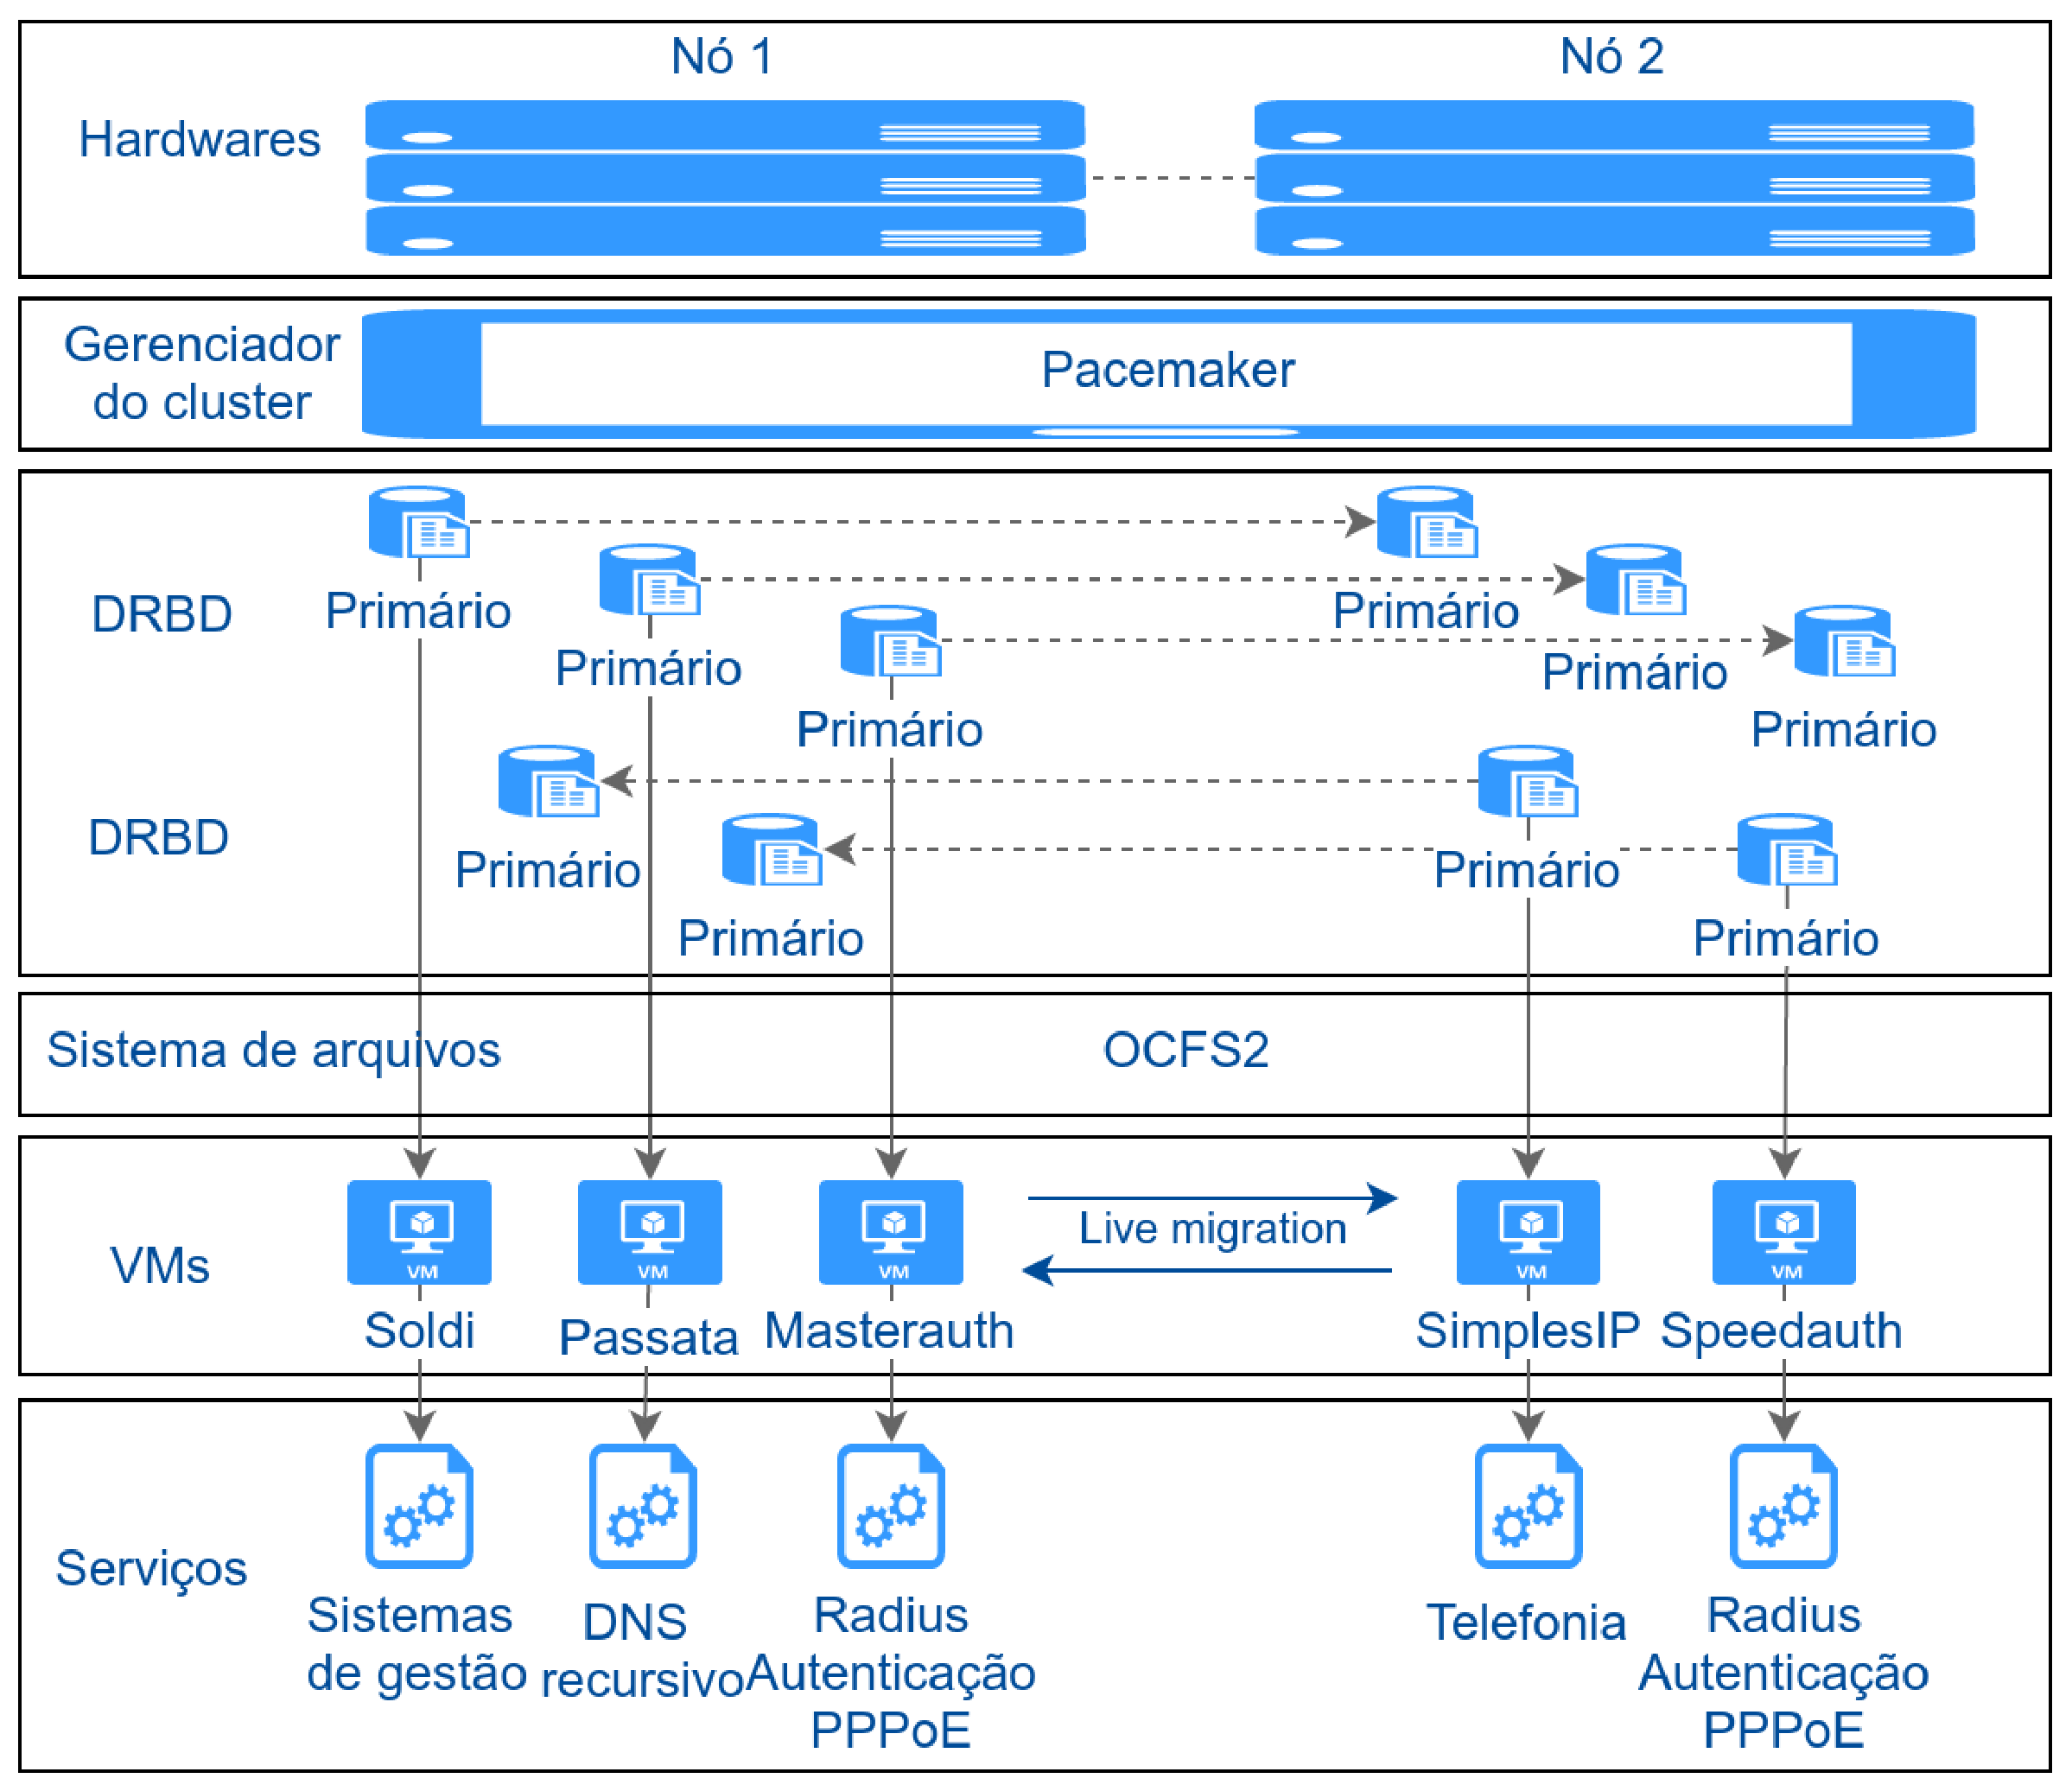
\includegraphics[width=350px]{img/projeto_estrutura.eps}
 \caption{Visão geral da estrutura do \textit{cluster}.}
 \label{fig:projeto_estrutura}
\end{figure}

\newpage
Já para a replicação de dados foi utilizado o \textit{software} \ac{DRBD}, que foi configurado no modo \textit{dual-master} onde os dois nós 
foram configurados como primários. Para tal configuração foi necessário utilizar um sistema de arquivos distribuídos que permite um acesso 
simultâneo e compartilhado aos dados, desta forma o \textit{software} adotado foi o \ac{OCFS2} \cite{ocfs2}. 
%Esse sistema de arquivos foi montado em um diretório dentro do sistema operacional dos nós, como por exemplo 
%\textit{/var/lib/libvirt/images}, sabendo que esse diretório contêm as imagens dos discos das \acp{VM}. 
Como pode ser observado na Figura \ref{fig:projeto_estrutura} todas alterações feitas em um disco de uma \ac{VM} é replicada para o 
outro nó através do \textit{software} \ac{DRBD}. 

Como pode-se também observar na Figura \ref{fig:projeto_discos} todas as operações de escritas realizadas são replicadas no outro nó do
\textit{cluster}, através do \textit{software} \ac{DRBD} e do \ac{OCFS2}. Cada dispositivo \ac{DRBD} é composto por um disco 
rígido\footnote[1]{Esse disco rígido pode ser composto por um conjunto de discos rígidos físicos configurados através de um \ac{RAID}.} 
(sda). Já o sistema de arquivos \ac{OCFS2} (quadro pontilhado) abrange os dois dispositivos \ac{DRBD}, desta forma permitindo o acesso simultâneo aos dados. 
%Para melhor entender o armazenamento e a replicação de dados criou-se a Figura \ref{fig:projeto_discos}, onde tem-se um dispositivo \ac{DRBD}
%em cada nó que faz a replicação de dados através da rede. Dentro de cada dispositivos \ac{DRBD} existe um disco rígido\footnote[1]{Esse disco 
%rígido é composto por um conjunto de discos rígidos físicos configurados através de um \ac{RAID}.} (sda). O quadro pontilhado que abrange os 
%dois dispositivos \ac{DRBD} e se estende pelos dois nós é o sistema de arquivos distribuídos \ac{OCFS2}, o qual permite o acesso simultâneo ao 
%dispositivo \ac{DRBD}. Esse sistema de arquivos é montado em um diretório do sistema operacional, desta forma permitindo o armazenamento 
%dos discos das máquinas virtuais. 
Os detalhes da instalação, da configuração do \ac{DRBD} e do sistema de arquivos \ac{OCFS2} estão detalhadas no Apêndice \ref{ap:confdisco}. 

\begin{figure}[h!]
 \centering
 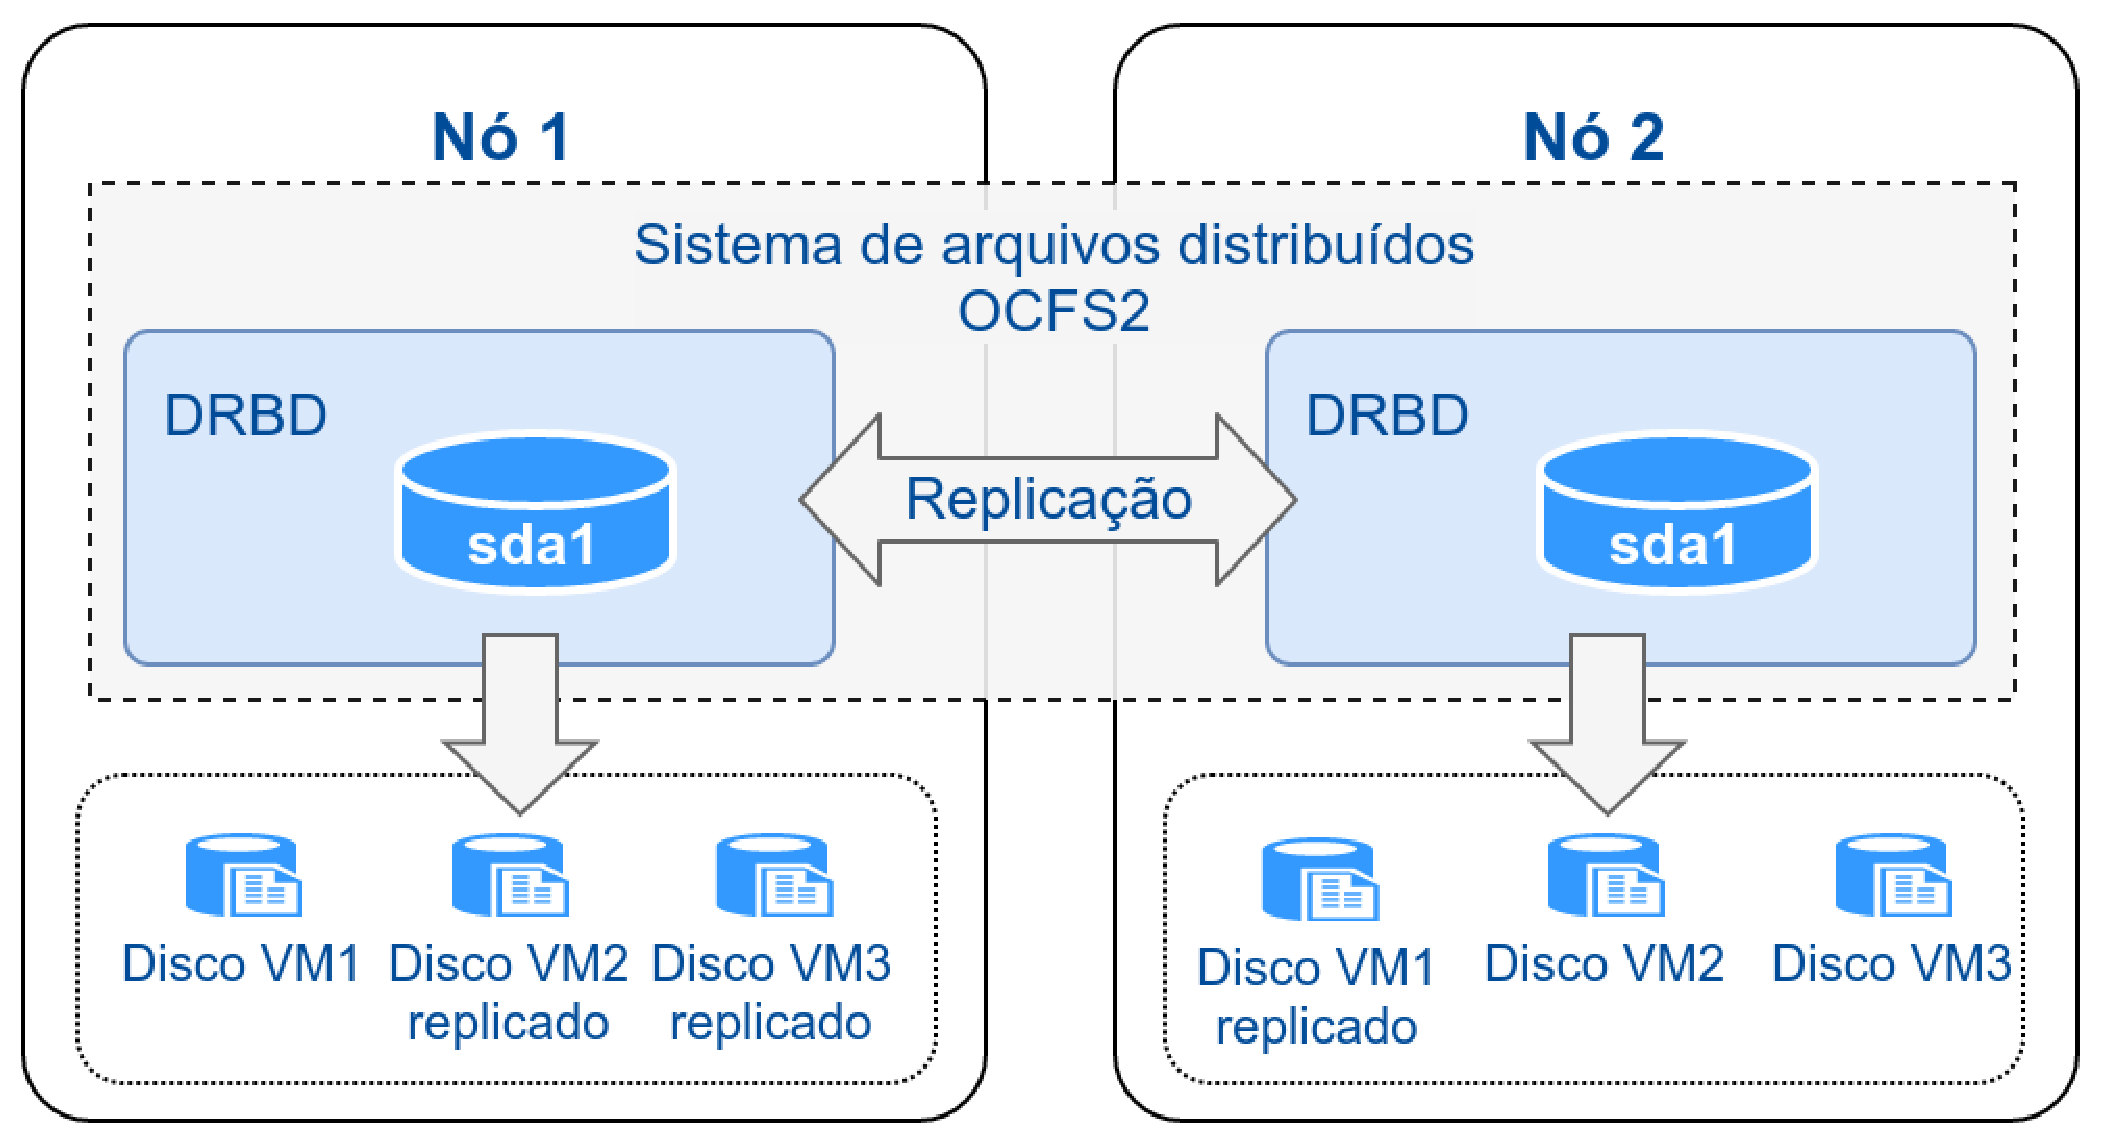
\includegraphics[width=320px]{img/projeto_discos.eps}
 \caption{Estrutura de armazenamento de dados do \textit{cluster}.}
 \label{fig:projeto_discos}
\end{figure}

%drbd
% O \ac{DRBD} será configurado no modo \textit{master-slave}, sendo que para cada disco das máquinas virtuais será criado um dispositivo de 
% replicação \ac{DRBD}. E para utilizar esse dispositivo como disco de uma máquina virtual será criado um volume lógico 
% \ac{LVM}\footnote{LVM é uma ferramenta de código aberto que possibilita a manipulação de discos rígidos, através da criação de grupos de volumes 
% e volumes lógicos para \textit{Linux}.} \cite{lvm}. 

\newpage
\section{Testes realizados}

A metodologia de testes adotada neste trabalho foi baseada nos trabalhos de \citet{reis2009} e \citet{goncalves2009}. No primeiro trabalho, 
o autor simulou as falhas de três formas distintas, que foram através do desligamento brusco do servidor, desligamento por \textit{software} e 
falha de rede. Já no segundo trabalho, foram realizados três testes, que foram a reinicialização do servidor físico, a migração de uma 
máquina virtual de forma manual, e por fim um teste de migração de uma \ac{VM} em tempo real (\textit{live migration}).
Neste trabalho optou-se por utilizar o teste de desligamento brusco e o desligamento por \textit{software} que foram utilizados por 
\citet{reis2009}. Já de \citet{goncalves2009}, utilizou-se o teste de migração em tempo real, porém adaptado para simular um agendamento de 
manutenção de \textit{hardware} ou de \textit{software}.
%, ou seja, migrar as \acp{VM} de um nó para outro utilizando a migração em tempo real, 
%com objetivo de fazer uma manutenção do sistema operacional deste nó.

%Os três testes descritos nas próximas seções foram efetuados no ambiente de alta disponibilidade com uma máquina virtual para fins de experimento, 
%devido ao fato destes testes possuírem risco de perda de dados durante a execução.
%Todavia, na Seção \ref{section:comparacaofinal} será feita a medição e a análise do período de um mês no ambiente de alta disponibilidade,
%sendo que neste ambiente estarão executando os serviços críticos definidos.

\subsection{Teste 1 - Desligamento físico}
%Desligamento físico (simulação falha de hardware ou elétrica): 4 vezes para medir tempo de downtime dos serviços e dos nodes (serviço não crítico)

Neste teste são simuladas falhas de \textit{hardware} ou falhas elétricas nos nós do \textit{cluster}, sendo que para isso foi feito o desligamento 
forçado de um nó do \textit{cluster}. Neste caso espera-se que os serviços sejam transferidos de forma automática para o outro servidor. 

A partir deste teste foi possível avaliar o processo de \textit{failover} dos serviços (máquinas virtuais) que estavam executando no nó que falhou, 
bem como medir o tempo de indisponibilidade dos serviços. Esse teste foi executado 10 vezes e o tempo de indisponibilidade foi medido utilizando o 
comando \textit{ping}. Para facilitar a medição foi utilizado um \textit{script} que encontra-se disponível no Apêndice \ref{ap:scriptindisp}. 
Desta forma, foi medido o tempo que o serviço ficou indisponível e o tempo que o servidor físico permaneceu indisponível.

Como pode ser observado na Tabela \ref{tab:teste1resultados} o tempo de indisponibilidade do serviço (máquina virtual) é de apenas 71,4 segundos, 
isso se deve ao fato da \ac{VM} ser iniciada em um nó secundário após o desligamento do principal. Só para exemplo de comparação, no caso de um 
servidor de virtualização que não possua esta solução de alta disponibilidade, o tempo para a recuperação do serviço seria igual a soma do 
tempo de inicialização do servidor físico mais o tempo de inicialização da máquina virtual, que totalizaria aproximadamente 151 segundos. 
%Além disso, o desvio padrão demonstra que existe pouca variação entre os tempos de indisponibilidade.
RELER ??

%Este teste juntamente com os dois testes das próximas seções foram efetuados no 
%ambiente de alta disponibilidade com uma máquina virtual para fins de experimento, por possuírem risco de perda de dados em sua execução.

% feito em 15/09 no ambiente de producao
% feito em 19/11, teste de 10 vezes no ambiente de teste nos notebook, fazer filmagem

\begin{table}[h!]
\caption{Resultados do teste de desligamento físico, contendo o tempo de indisponibilidade em segundos.}
\small
\label{tab:teste1resultados}
\begin{center}
\begin{tabular}{|l|l|l|}\hline
 & \textbf{Tempo de indisponibilidade (s)} & \textbf{Desvio padrão} \\\hline
Nó & 80,3 & 18,19 \\\hline
Máquina virtual & 71,4 & 14,93 \\\hline
\end{tabular}
\end{center}
\end{table}

Na pior das hipóteses, caso haja uma falha definitiva do servidor, sendo necessário reconfigurar a máquina virtual, reinstalar as aplicações,
configurá-las e restaurar o \textit{backup}, o \ac{MTTR} seria significativamente maior. Dependendo do servidor e da aplicação, 
a indisponibilidade poderia ser maior do que 24 horas.

%O procedimento deste teste é o seguinte:
%\begin{itemize}
% \item Acessar o terminal do servidor de monitoramento;
% \item Executar comando \textit{ping} e medir o tempo de indisponibilidade (\textit{script} no Apêndice \ref{ap:scriptindisp});
% \item Forçar desligamento do nó;
% \item Aguardar máquinas virtuais iniciarem no outro nó;
% \item Finalizar a medição do tempo e \textit{ping}.
%\end{itemize}

% A Figura \ref{fig:teste1_disponibilidade} demonstra a disponibilidade dos servidores físicos Nó 1 (\textit{Brina}) e Nó 2 (\textit{Piova}) e da 
% máquinas virtual (\textit{Trapel}). A máquina virtual teve apenas 1 minuto e 10 segundos de \textit{downtime}, deste modo, caso o 
% \textit{hardware} no qual a máquina virtual está executando falhe, o serviço será reestabelecido neste curto período de tempo.
% 
% \begin{figure}[h!]
%  \centering
%  \includegraphics[width=470px]{img/teste1_disponibilidade.eps}
%  \caption{Disponibilidade servidores físicos \textit{Brina} e \textit{Piova} e da máquina virtual \textit{Trapel}.}
%  \label{fig:teste1_disponibilidade}
% \end{figure}


\subsection{Teste 2 - Desligamento por software}

Esse teste simula falhas de \textit{software} nos nós do \textit{cluster}. Neste caso, pode-se citar como exemplo, uma falha no \textit{software} 
de virtualização, com isso o nó não conseguiria iniciar a máquina virtual. Esse tipo de situação também pode ocorrer em uma falha de atualização 
do sistema operacional ou de \textit{kernel}.
Nestes tipos de falhas, os serviços devem ser transferidos para o outro nó de forma automática, reduzindo assim a indisponibilidade desses serviços. 
%Desta forma, pode-se validar o processo de \textit{failover} dos serviços que estavam executando no nó que apresentou a falha.

Para simular a falha, os nós foram acessados via \ac{SSH} e foi executado o comando \textit{reboot}. Esse teste foi executado 10 vezes e o 
tempo de indisponibilidade foi medido da mesma forma do que o teste anterior, ou seja, utilizando o comando \textit{ping}, sendo que foi medido 
o tempo de indisponibilidade do nó e da máquina virtual. A Tabela \ref{tab:teste2resultados} apresenta o tempo de indisponibilidade e o 
desvio padrão do nó e da \ac{VM}. Pode-se observar que o tempo de indisponibilidade da \ac{VM} é consideravelmente menor que o tempo do 
servidor físico, pois a \ac{VM} foi iniciada no nó secundário logo após a simulação da falha no nó principal. 
De fato, ele representa apenas 1/6 do tempo de indisponibilidade do servidor físico que é de 58,5 segundos. 
RELER ??

% feito em 09/09 no ambiente de producao
% feito em 19/11, teste de 10 vezes no ambiente de teste nos notebook

% O procedimento deste teste é o seguinte:
% \begin{itemize}
%  \item Acessar o terminal do servidor de monitoramento;
%  \item Executar comando \textit{ping} e medir o tempo de indisponibilidade (\textit{script} no Apêndice \ref{ap:scriptindisp});
%  \item Acessar o terminal do nó que será reiniciado;
%  \item Executar o comando \textit{reboot};
%  \item Aguardar máquinas virtuais iniciarem no outro nó e aguardar retorno do nó reiniciado;
%  \item Finalizar a medição do tempo e \textit{ping}.
% \end{itemize}

\begin{table}[h!]
\caption{Resultados do teste de desligamento por \textit{software}, com tempo de indisponibilidade em segundos e o desvio padrão.}
\small
\label{tab:teste2resultados}
\begin{center}
\begin{tabular}{|l|l|l|}\hline
 & \textbf{Tempo de indisponibilidade (s)} & \textbf{Desvio padrão} \\\hline
Nó & 58,5 & 1,58 \\\hline
Máquina virtual & 11 & 3,16 \\\hline
\end{tabular}
\end{center}
\end{table}

Há alguns meses ocorreu um problema semelhante a este teste em um servidor de virtualização, que foi atualizado de forma automática. Neste caso, 
ocorreu um erro na atualização e o servidor não inicializou corretamente. Os serviços executados nele ficaram aproximadamente 
6 horas indisponíveis. Através da solução implementada esse tempo seria de apenas 11 segundos, pois a \ac{VM} seria iniciada no outro nó. 

\subsection{Teste 3 - Manutenção agendada}
%Agendamento de manutenção (reboot para atualização de software): 2 semanas ou mais, 1 manutenção por semana, com live migration, reboot e 
%atualização de kernel dos nodes. Resultados: latência, comparação downtime servidor virtual e físico

% feito em 17/09 a 30/09
% crontab brina:
% */10 04 * * 2 /usr/local/sbin/script_pacemaker_manutencao.sh
% crontab piova:
% */10 04 * * 4 /usr/local/sbin/script_pacemaker_manutencao.sh
% crontab monit:
%59 03 * * 2 cd /home/bruno/pacemaker/teste2/; bash indisponibilidade.sh 186.195.16.14 1
%59 03 * * 2 cd /home/bruno/pacemaker/teste2/; bash indisponibilidade.sh 186.195.16.13 1
%59 03 * * 4 cd /home/bruno/pacemaker/teste2/; bash indisponibilidade.sh 186.195.16.6 2
%59 03 * * 4 cd /home/bruno/pacemaker/teste2/; bash indisponibilidade.sh 186.195.16.13 2

Reinicializações são necessárias para manutenções de \textit{hardware}, atualização de \textit{software} e até mesmo para 
rejuvenescimento\footnote{O rejuvenescimento de \textit{software} consiste nas aplicações de métodos para remover problemas gerados pelo 
envelhecimento. Um exemplo de um método é o \textit{reboot} de um sistema operacional, uma vez que esse torna-se suscetível a gerar erros e 
falhas.} de \textit{software} \cite{melo2014}. Desta forma, esse teste foi realizado de forma a simular manutenções previamente agendadas.
Esse teste consiste no agendamento de 4 manutenções efetuadas durante o período de 13 dias, para tanto, criou-se um \textit{script} que é 
responsável por migrar as \acp{VM} de um nó e posteriormente reiniciá-lo. Este \textit{script} está disponível no Apêndice 
\ref{ap:scriptmanutencao}. Para o agendamento e a execução deste \textit{script} foi utilizada a ferramenta \textit{crontab} do \textit{Linux}
\cite{neves2008}. 

Observa-se na Tabela \ref{tab:teste3resultados} que o tempo de \textit{downtime} da máquina virtual é praticamente nulo, ou seja, 
não houve indisponibilidade nos serviços devido a migração em tempo real da \ac{VM}. 
Já nos nós tem-se um tempo de indisponibilidade de 145,5 e 173 segundos devido a reinicialização dos mesmos.
Também pode-se observar o percentual de disponibilidade da \ac{VM} e dos nós do \textit{cluster} medidos durante o período de 13 dias.
Destaca-se que a máquina virtual não apresentou nenhuma indisponibilidade. Essa disponibilidade foi obtida através da ferramenta 
\textit{Nagios} \cite{nagios} da empresa.

\begin{table}[h!]
\caption{Resultados do teste de manutenção agendada, com o tempo de indisponibilidade em segundos e a disponibilidade medida no período de 13 dias.}
\small
\label{tab:teste3resultados}
\begin{center}
\begin{tabular}{|l|p{7cm}|p{4cm}|}\hline
 & \textbf{Tempo de indisponibilidade média} & \textbf{Disponibilidade} \\\hline
Nó 1 & 145,5 & 99,976\% \\\hline
Nó 2 & 173 & 99,975\% \\\hline
Máquina virtual & 0 & 100\% \\\hline
\end{tabular}
\end{center}
\end{table}

%O procedimento deste teste é o seguinte:
%\begin{itemize}
% \item Executar comando \textit{ping} e medir o tempo de indisponibilidade (\textit{script} no Apêndice \ref{ap:scriptindisp});
% \item Executar o \textit{script} que desativa o nó (comando \textit{standby}) e executa o \textit{reboot} (Apêndice \ref{ap:scriptmanutencao});
% \item Após retorno do nó executar novamente o \textit{script} anterior para retorno do nó ao \textit{cluster};
% \item Finalizar a medição do tempo e \textit{ping}.
%\end{itemize}

%A Figura \ref{fig:teste2_trapel1} demonstra a disponibilidade da máquina virtual, onde pode-se perceber que não houve nenhuma indisponibilidade. 
%Esses dados foram produzidos pela ferramenta \textit{Nagios} \cite{nagios}, que faz o monitoramento da empresa. 
%gráfico comparativo nagios da disponibilidade do servidor fisico e do virtual
%gráfico nagios - Trends(gráfico) ou Availability (resumo) - Hosts - servidor - tempo 18/09 a 30/09 + Include Soft States = yes
% \begin{figure}[h!]
%  \centering
%  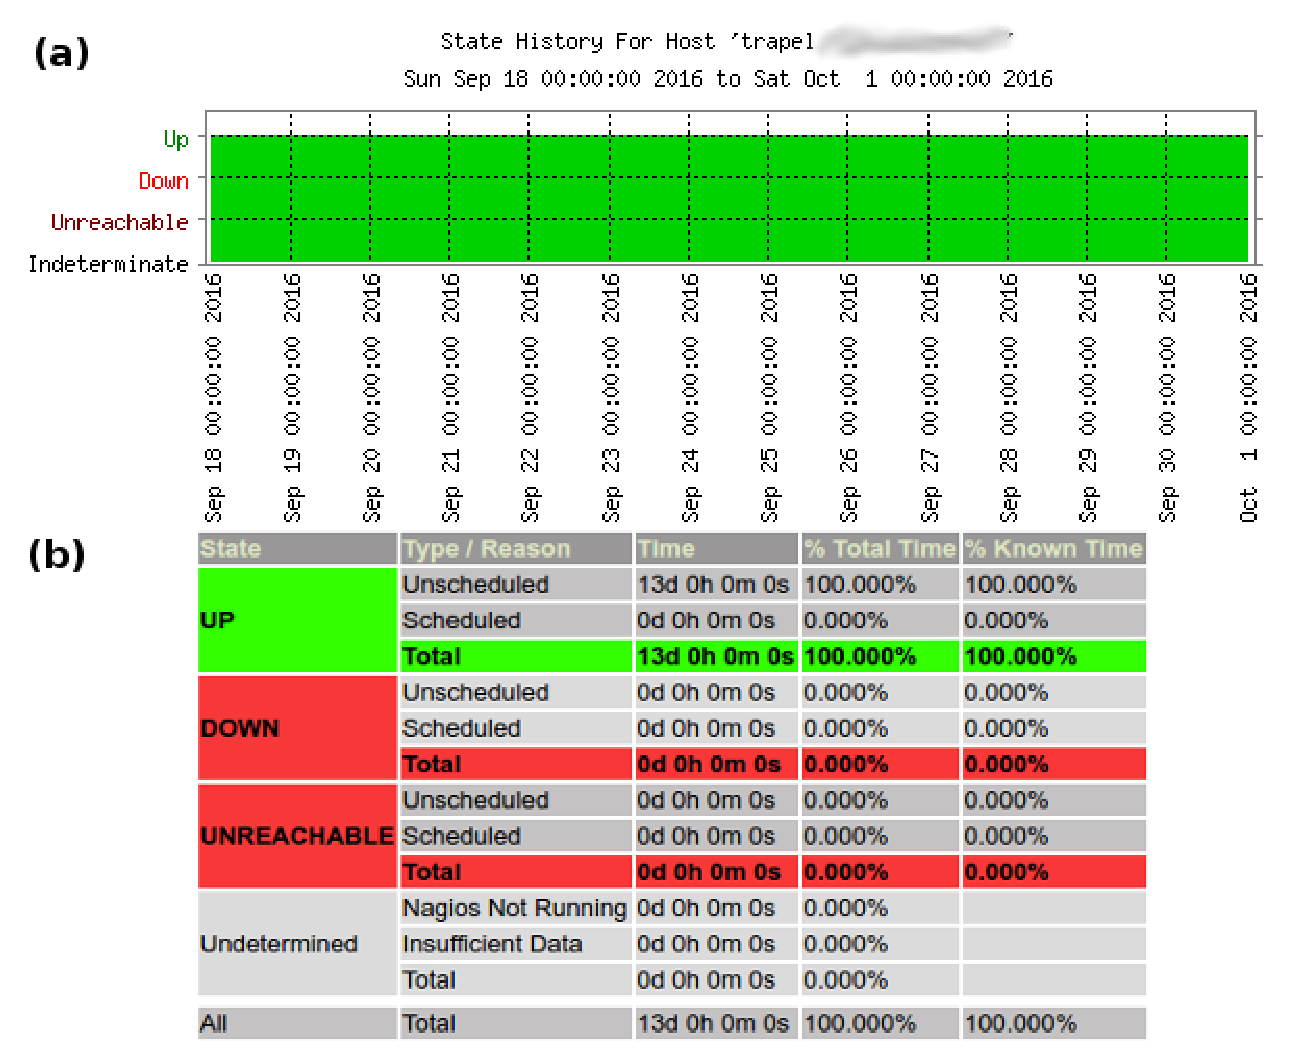
\includegraphics[width=360px]{img/teste2_trapel1.eps}
%  \caption{Disponibilidade da máquina virtual, com o gráfico da disponibilidade (a) e a tabela com detalhes de tempo e percentual (b).}
%  \label{fig:teste2_trapel1}
% \end{figure}

%Comparando os resultados da máquina virtual (Figura \ref{fig:teste2_trapel1} (b)) com os resultados dos nós 1 e 2 (Figura \ref{fig:teste2_brina1} 
%(b) e Figura \ref{fig:teste2_piova1} (b)), pode-se perceber a diferença do \textit{uptime}, que fica entre 99,975\% e 99,976\% para os nós e 
%100\% para a máquina virtual. Já nos gráficos da Figura \ref{fig:teste2_brina1} (a) e da Figura \ref{fig:teste2_piova1} (a), pode-se observar 
%as duas reinicializações feitas.
% \begin{figure}[h!]
%  \centering
%  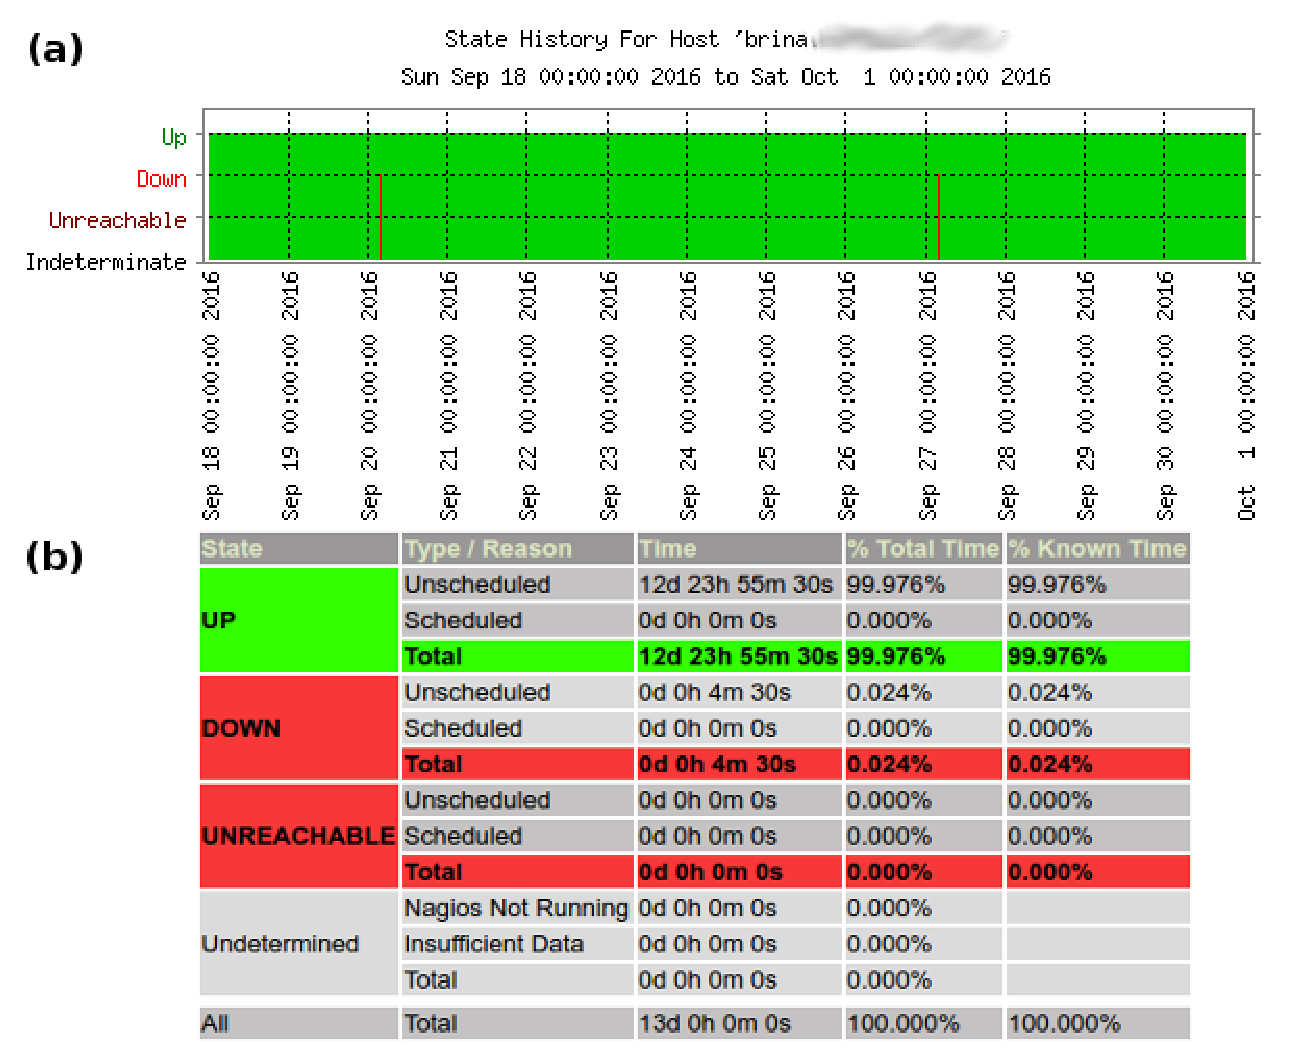
\includegraphics[width=360px]{img/teste2_brina1.eps}
%  \caption{Disponibilidade do Nó 1, com o gráfico da disponibilidade (a) e a tabela com detalhes de tempo e percentual (b).}
%  \label{fig:teste2_brina1}
% \end{figure}
% 
% \begin{figure}[h!]
%  \centering
%  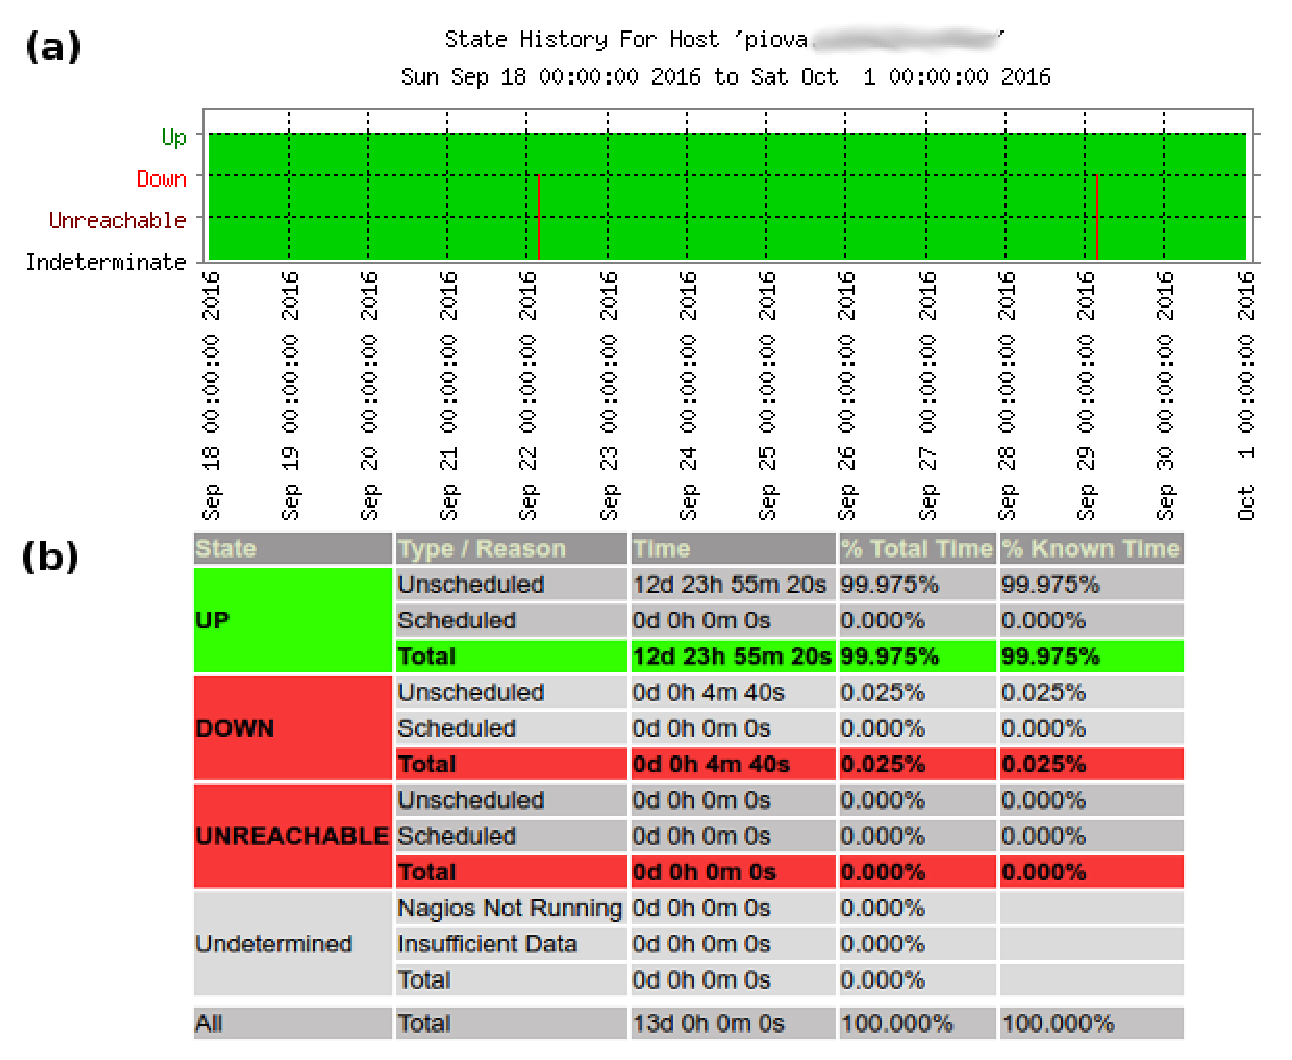
\includegraphics[width=360px]{img/teste2_piova1.eps}
%  \caption{Disponibilidade do Nó 2, com o gráfico da disponibilidade (a) e a tabela com detalhes de tempo e percentual (b).}
%  \label{fig:teste2_piova1}
% \end{figure}

Observa-se que durante o processo de \textit{live migration} de uma \ac{VM} de um nó para outro, a latência da máquina virtual aumentou, 
sendo que a latência, em uma rede de computadores, é o tempo que um pacote leva para chegar ao destino \cite{geordano2014}.
O aumento da latência ocorre devido ao fato da transferência da \ac{VM} ser feita através da rede, a qual é necessária para a cópia da memória 
durante a migração em tempo real da máquina virtual. ?? VER
Esse aumento na latência pode ser observado na Figura \ref{fig:teste2_latencia}, no intervalo de tempo de 50 a 100 segundos.

%1) Aumento de trafego na rede
%2) Algum aumento da carga computacional do nodo destino.
%?? por causa da transferencia da memoria atraves da rede.

%Mesmo com o aumento de latência não ocorre perda significante de desempenho durante a migração da máquina virtual.
%teste2/186.195.16.13-stat-1.log
%teste2/186.195.16.13-stat-2.log

\begin{figure}[h!]
 \centering
 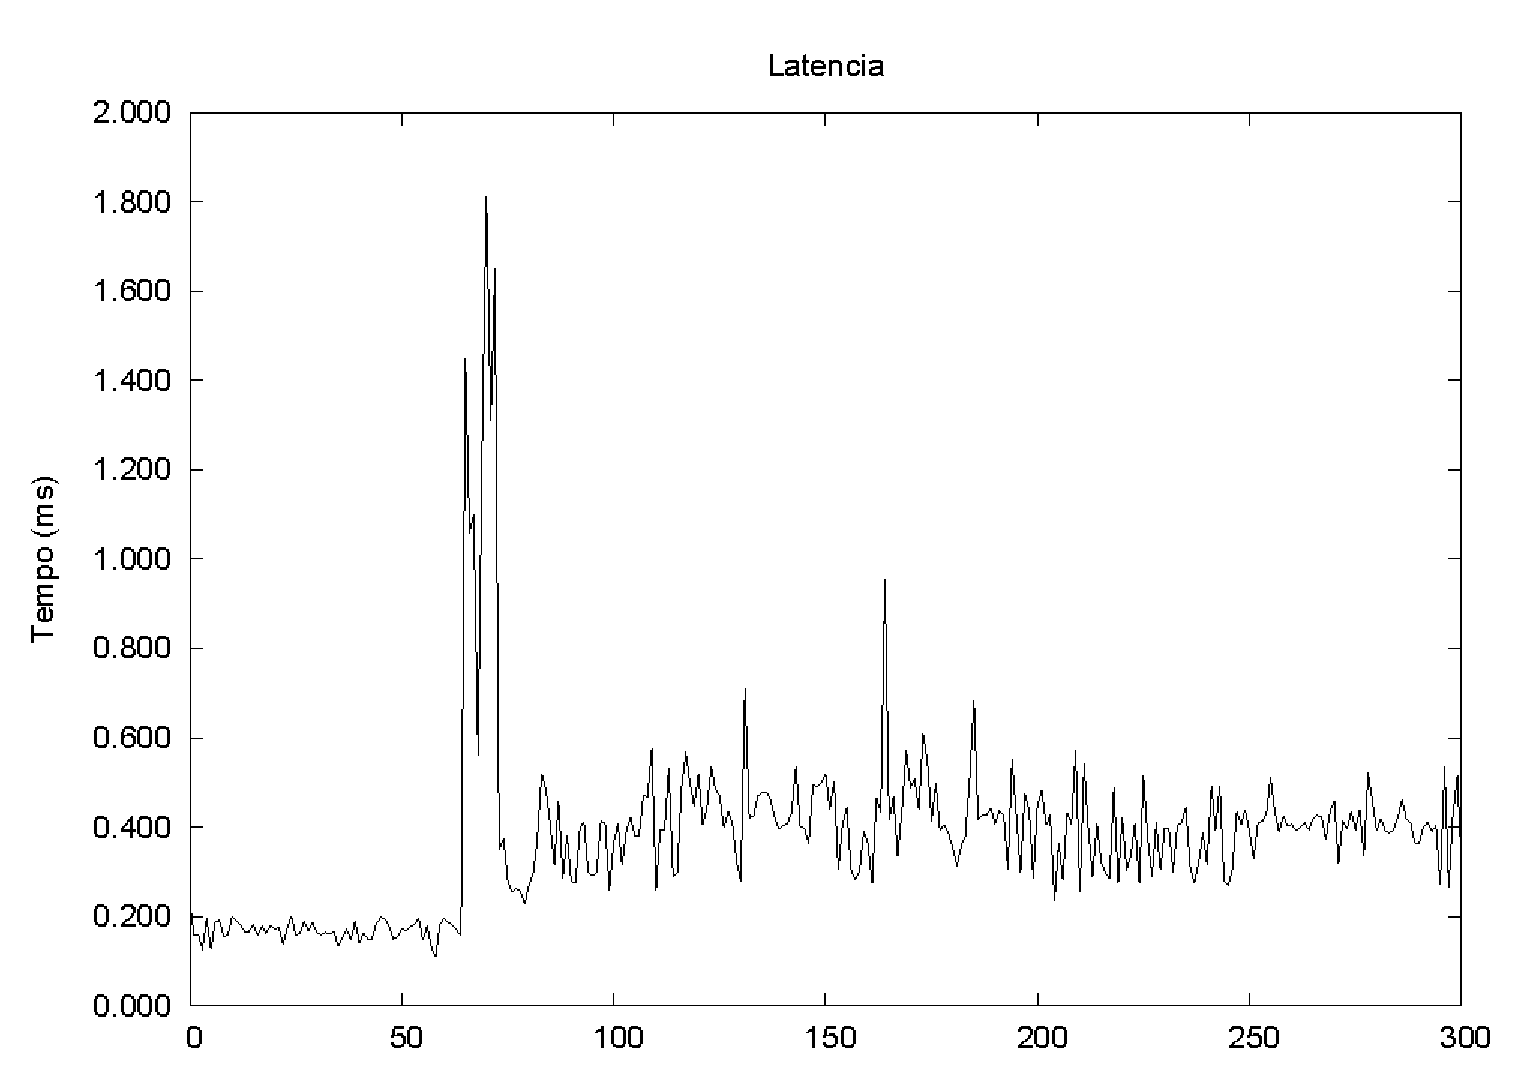
\includegraphics[width=320px]{img/teste2_latencia.eps}
 \caption{Latência da máquina virtual durante o \textit{live migration}.}
 \label{fig:teste2_latencia}
\end{figure}

\newpage
\section{Cálculo da disponibilidade}
\label{section:comparacaofinal}
%Medição da disponibilidade dos serviços críticos por 30 dias (14/10 a 12/11) FAZER uma manutenção de hardware.
%Comparar ao mês de setembro (01/09 a 30/09) no ambiente antigo com uma reinicialização dos servidores físicos (reiniciados em 06/09/16)

Esta seção apresenta uma comparação da disponibilidade entre o ambiente antigo e o ambiente de alta disponibilidade. 
Para tanto, foi feita uma medição da disponibilidade do período de um mês no ambiente antigo e de um mês no ambiente de alta disponibilidade, 
nos quais executavam os serviços críticos. Porém, para se obter resultados mais consistentes seria interessante realizar uma mensuração mais longa, 
com duração entre 6 meses e 1 ano. Contudo, isso tornou-se inviável devido ao tempo disponível para a implementação deste trabalho. 
%Nestes ambientes encontravam-se executando os serviços críticos que foram definidos na Seção \ref{section:maqservcrit}. 

A Tabela \ref{tab:testefinal} apresenta a disponibilidade de cada serviço crítico, tanto no ambiente antigo quanto 
no ambiente de alta disponibilidade que foi criado. Pode-se observar que a disponibilidade máxima dos serviços no antigo ambiente é de 
três noves. já no ambiente de alta disponibilidade tem-se uma disponibilidade próxima a 100\% para todos os serviços.
Além disso, a tabela apresenta o tempo de indisponibilidade de cada serviço. Observa-se que o ambiente de alta disponibilidade apresentou
somente uma indisponibilidade de 1 minuto e 40 segundos no serviço de \ac{DNS}. Essa indisponibilidade ocorreu devido a um problema de segurança,
DDoS.
O restante dos serviços não apresentaram indisponibilidade durante o período medido.
RELER ??

%graficos: nagios_disponibilidade1_*
\begin{table}[h!]
\caption{Disponibilidade e tempo de indisponibilidade (em minutos) do antigo ambiente e do novo ambiente de alta disponibilidade, que foram medidos no período de um mês.}
\small
\label{tab:testefinal}
\begin{center}
\begin{tabular}{|l|p{2cm}|p{2cm}|p{2cm}|p{2cm}|}\hline
 & \multicolumn{2}{|c|}{\textbf{Disponibilidade}} & \multicolumn{2}{|c|}{\textbf{Tempo de indisponibilidade}} \\\hline
\textbf{Serviço} & \textbf{Antigo ambiente} & \textbf{Novo ambiente} & \textbf{Antigo ambiente} & \textbf{Novo ambiente} \\\hline
DNS recursivo & 99,978\% & 99,996\% & 9:40 & 1:40 \\\hline
Autenticação \ac{PPPoE} & 99,936\% & 100\% & 27:40 & 0 \\\hline
Autenticação \ac{PPPoE} & 99,930\% & 100\% & 30:20 & 0 \\\hline
Sistemas & 99,913\% & 100\% & 37:20 & 0 \\\hline
Telefonia & 99,866\% & 100\% & 58:0 & 0 \\\hline
\end{tabular}
\end{center}
\end{table}


\section{Considerações finais}

Neste capítulo foi apresentada a arquitetura de alta disponibilidade que foi implementada neste trabalho, sendo que essa solução é baseada em
um ambiente de \textit{cluster} composto por dois servidores físicos, onde foram configuradas máquinas virtuais contendo os serviços 
críticos da empresa. Para a criação desta estrutura utilizou-se um \textit{software} para o gerenciamento do \textit{cluster} e um 
para a replicação de dados, que foram o \textit{Pacemaker} e o \ac{DRBD}, respectivamente.

Após a implementação, foram feitos testes que apresentaram uma redução no tempo de indisponibilidade dos serviços críticos. 
De fato, os testes realizados permitiram validar o ambiente de alta disponibilidade e permitiram concluir que é possível criar um ambiente 
de alta disponibilidade baseado no uso de \textit{software} livre. 
Porém, destaca-se que seria necessário mais tempo para efetuar medições mais precisas e concisas.
RELER ??

%Para possibilitar a medição dos dados de disponibilidade foi utilizado \textit{scripts} e o comando \textit{ping}, além da ferramenta de 
%monitoramento da empresa (\textit{Nagios}). Com o tempo de indisponibilidade do antigo ambiente e do ambiente de alta disponibilidade criado,
%pôde-se comparar esses dois ambientes.
